%% Submissions for peer-review must enable line-numbering 
%% using the lineno option in the \documentclass command.
%%
%% Preprints and camera-ready submissions do not need 
%% line numbers, and should have this option removed.
%%
%% Please note that the line numbering option requires
%% version 1.1 or newer of the wlpeerj.cls file.

\documentclass[fleqn,10pt,lineno]{wlpeerj} % for journal submissions
% \documentclass[fleqn,10pt]{wlpeerj} % for preprint submissions

\title{Analysis of Altmetrics Publications and Tweets}

\author[1]{Stefan Kasberger}
\affil[1]{Karl Franzens University of Graz}

\keywords{Open Science, Altmetrics, Twitter}

\begin{abstract}
The fast increase of scientific content needs new approaches to evaluate the quality and content. Next to this it also needs new ways to communicate the results to the public and to the scientific communities who could be interested in it. Altmetrics offers new ways to measure the impact of results and Twitter makes sharing easy. The first analysis looks for patterns in the Altmetrics of publications, the second is looking for patterns in communication on twitter around the topic of Altmetrics.
\end{abstract}

\begin{document}

\flushbottom
\maketitle
\thispagestyle{empty}

\section*{Introduction}

\subsection*{Altmetrics of Arxiv Papers}

The body of scientific literature is growing immensely since the last 400 years and reached a yearly growth rate of 8 to 9\% in 2012 \citep{Bornmann2014}. This huge growth of knowledge needs new ways to understand and evaluate the scientific outputs and to support the scientific community with this task \citep{Costas2014}. Altmetrics stands for alternative metrics and expand the traditional way of evaluation through citations with additional metrics, like mentions on Twitter, Facebook, Blogs, Google+ and others to enrich the quantitative analysis. Altmetric try to establish a new way to evaluate the impact of scientific content to the public and the scientific community and to offer a more transparent and open aproach to evaluation, than the actually used impact factor. The following analyses looks for patterns regarding altmetrics in the ten most cited publications on twitter, which relate to the term "Social Network Analysis" from the open access repository ArXiv.

\subsection*{Twitter Mentions of \#altmetrics14}

Social media gets more and more important to disseminate scientific knowledge in general and publications in special \citep{Moriano2014}, with big differences between disciplines \citep{Haustein2014}. To better understand the dynamics of knowledge dissemination in the scholarly communities, the Twitter analysis looks for patterns in the tweets with the hashtag \#altmetrics14.

\section*{Methods}    
   
\subsection*{Altmetrics of Arxiv Papers}
To retrieve, compute and plot the data, the statistical programming language R with the rAltmetric and aRxiv packages were used. First the Arxiv API was queried with the terms "Social", "Network" and "Analysis" with a limit of 1000 results. Then the ones without DOI were filtered out and saved. After this, the altmetrics of all papers left were computed. The results then were ranked after "cited\_by\_tweeters\_count" and the ten publications with the most counts were taken. The results were plotted and exported as CSV. The original 8th ranked publication had to be removed, because the altmetric plot made some visualization problems.

\subsection*{Twitter Mentions of \#altmetrics14}
The twitter dataset used from \cite{ernesto_altmetrics14_2014} first had to be transformed into another data-format for easier use (CSV). To get the data in the wanted structure of "tweeters" and "mentioned", it first must be extracted from the CSV file. The "tweeters" are the twitter user who created the tweet and are stored in the column "from\_user". The "mentioned" are the twitter user mentioned by the "tweeter" directly in a tweet, typically with "@username". It is stored inside the "entities\_str" column, a JSON object with a list of the mentioned users (user\_mentions) with their user name (screen\_name). Retweets are filtered out through two regular expressions, so they do not skew the outcome. This results 1009 mentions, which are then plotted as a grid of frequencies \citep{tweets_tutorial} and a density function to make interpretation easy. Because of the usual power-law distribution of tweets\citep{Moriano2014}, the data was scaled logarithmically to make visual exploration easier.

\section*{Results}

\subsection*{Altmetrics of Arxiv Papers}

\begin{table}[ht]
\centering
\begin{tabular}{c|p{8cm}|c|c|c}
Rank & Publication & Twitter & Facebook & Google+ \\\hline
1 & The Twitter of Babel: Mapping World\newline Languages through Microblogging Platforms & 2563 & 5 & 13 \\
2 & A Principal Component Analysis of 39 Scientific Impact Measures & 292 & 3 & 5 \\
3 & Dynamics of Conflicts in Wikipedia & 177 & 2 & 6 \\
4 & Early Prediction of Movie Box Office Success Based on Wikipedia Activity Big Data & 125 & 3 & 4 \\
5 & World citation and collaboration networks: uncovering the role of geography in science & 105 & 9 & 3 \\
6 & Assessing Vaccination Sentiments with Online Social Media: Implications for Infectious Disease Dynamics and Control & 115 & NA & 1 \\
7 & Persistence of social signatures in human communication & 108 & 2 & 2 \\
8 & A large-scale community structure analysis in Facebook & 83 & 1 & 5 \\
9 & Predicting human preferences using the block structure of complex social networks & 90 & 2 & 5 \\
10 & Is Europe Evolving Toward an Integrated Research Area? & 76 & 2 & NA
\end{tabular}
\caption{\label{tab:altmetrics}The top 10 tweeted publications from Arxiv regarding the terms "Social" "Network" "Analysis" with further alternative metrics (Altmetrics).}
\end{table}

\begin{figure}[ht]\centering
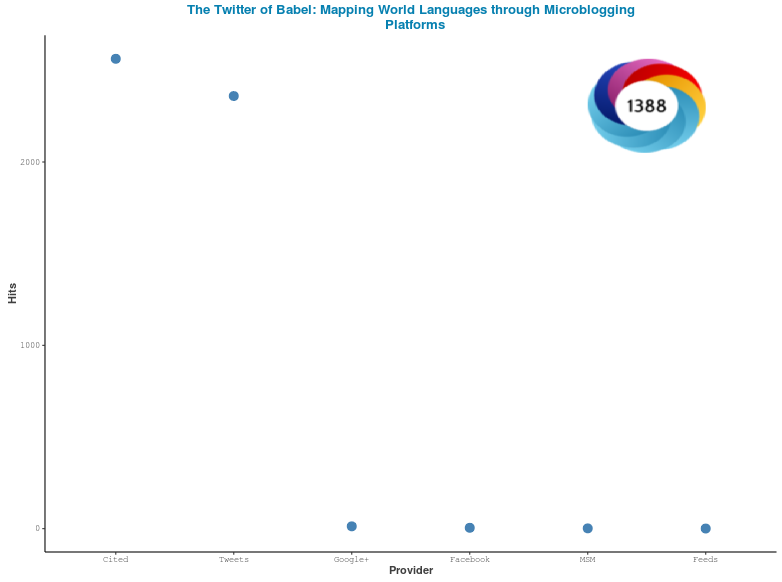
\includegraphics[width=10cm]{altmetrics-01.png}
\caption{Altmetrics plot of the top publication "The Twitter of Babel: Mapping World Languages through Microblogging Platforms".}
\label{fig:altmetrics-01}
\end{figure}

The Arxiv query returned 276 publications with DOI's, so a little bit more than on quarter of the queried publications (1000) had some altmetrics. This means, that most of the publications do not have even one single citation on the web, and so is nearly invisible for others. 64 of publications with metrics had Facebook citations and 54 were mentioned on Google+. Only two publications had no citation on twitter. Google+, which has a way smaller user base than Facebook, is more often used. The most cited paper on Twitter leads with 2563 cites by nearly a magnitude compared to the following one with 292 citations. This could be, because as the title of "The Twitter of Babel: Mapping World Languages through Microblogging Platforms" is about Twitter itself, based on the assumption, that the scientific community who is doing research about Twitter is over-proportionally on Twitter and also uses it more intense. In general, the number of Twitter citations is way bigger than the mentions on Facebook (5 citations) and Google+ (13 citations). 

\subsection*{Twitter Mentions of \#altmetrics14}

\begin{figure}[ht]\centering
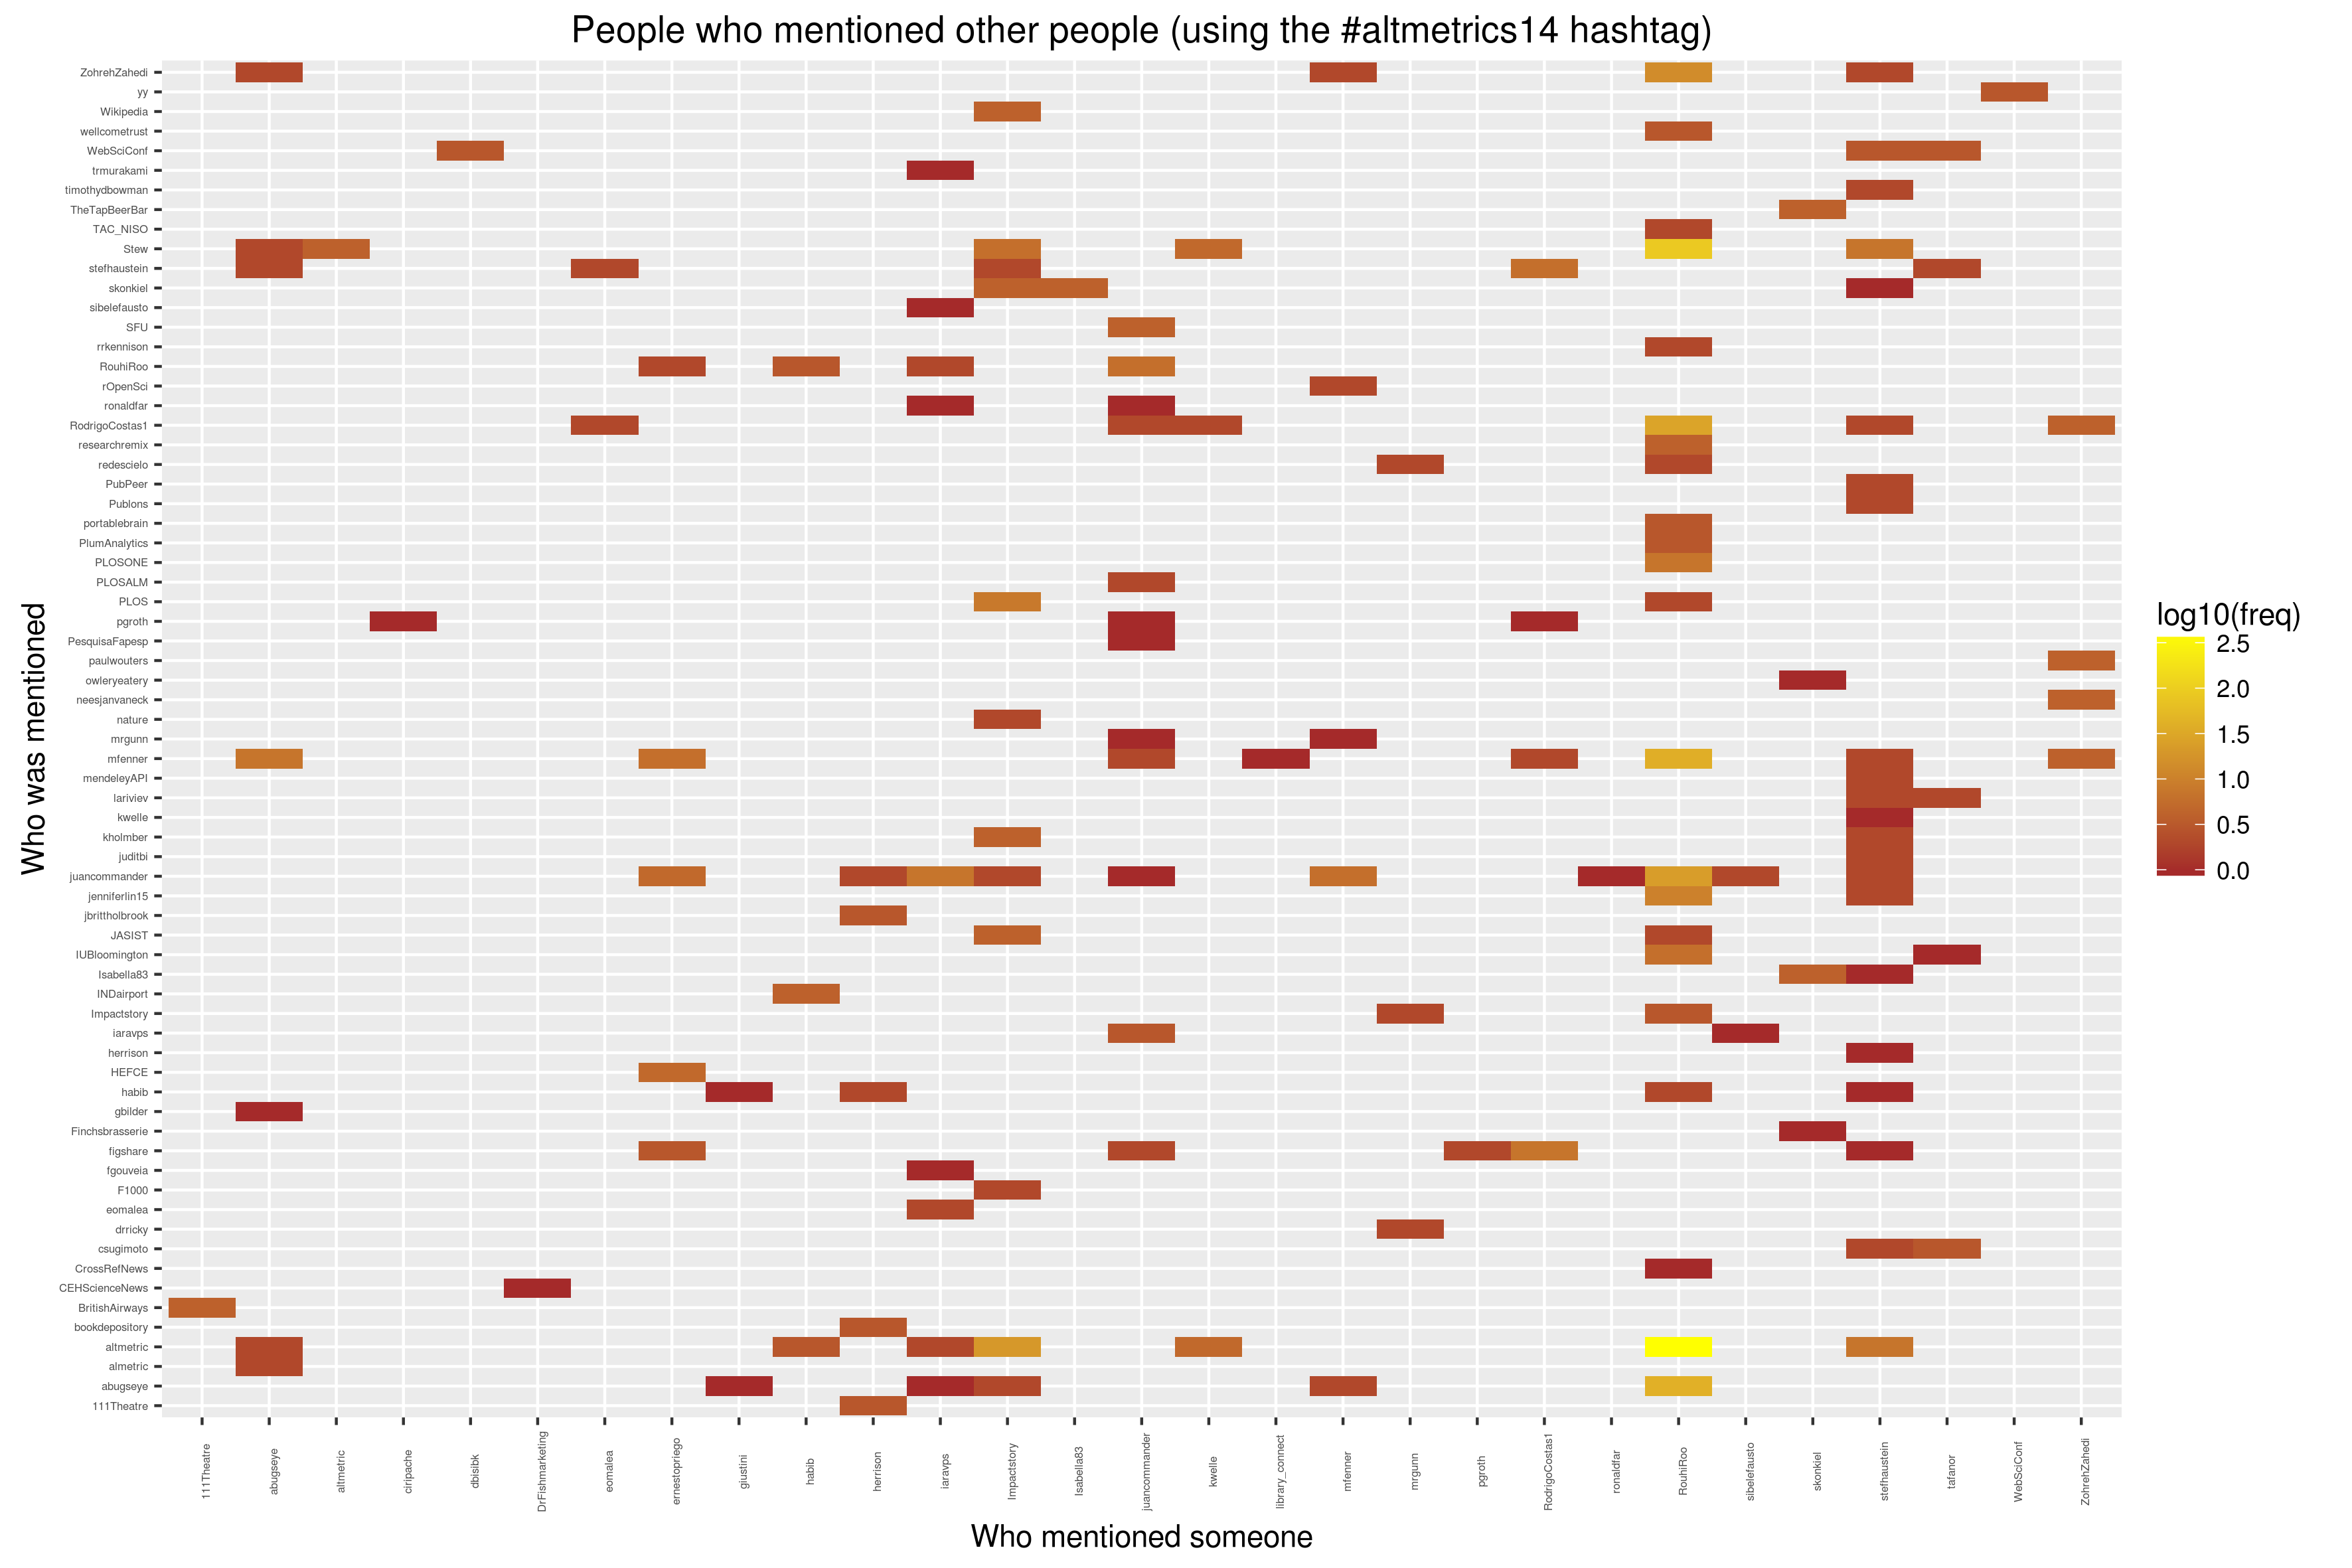
\includegraphics[width=\linewidth]{altmetrics14_mentions-2.png}
\caption{Grid with the frequency how often a Twitter user directly mentions another user. The scale is logarithmically transformed.}
\label{fig:twitter-mentions}
\end{figure}

The social network analysis of the data from \#altmetrics14 show the usual power-law distribution regarding re-occuring direct communication. As you can see from the grid plot (Figure 2), most of the tweets are done by a very few ones, and also most of the mentioned are addressed to just a small share of the whole user set. 

The user "@RouhiRoo" is with 677 direct mentions of other twitter accounts an extreme outlier and by far the user with the most direct mentions of others in the dataset; but only got mentioned 13 times by another user. It also has the by far biggest number in direct mentions to one and the same user (@altmetris) with 398 times mentioned in a tweet. This means, that on average, "@RouhiRoo" mentioned "@altmetrics" directly in over every second tweet with \#altmetrics14, followed on second place also by "@RouhiRoo with 84 re-occuring direct mentions of "@Stew". The related Twitter profile states "@altmetric product specialist" in the description. With 3,851 tweets in total till January 2016, nearly every sixth tweet used so far the hashtag \#altmetrics14 and included a direct mention of someone else, which is a huge share. 
Another finding is, that institution (e. g. PLOS, Fighshare, Altmetrics, WebSciConf) are more often mentioned than they themselves mention other twitter users. This also makes sense, because a lot of the institutions mentioned, stand for an organisation connected to the topics of altmetrics, Open Access or scholarly communication and therefore carry special value for users.

\section*{Conclusion and Future Work}

Both analysis are just first views into the field of social network analysis and scientometrics, but they show one important familiarity: the metrics only matter in context. Altmetrics do not itself tell the story or the context, the outcomes always must be evaluated also by humans.

In terms of communication, Twitter leads by far compared to other services like Google+ and Facebook in academia. But also here, the context is of very importance. Self-referential mechanisms can skew the data as seen in the Twitter publication. Another interesting finding is, that Google+ is over-proportionally used in academia, compared to the whole public. 

It is also clearly visible, that the idea of Open Science is in it's early stage and needs a lot of effort by researchers, funders and the scientific communities itself that it can deliver what it promises. Dirty bibliometric data, unstable software and missing methodological framework and case studies make application of this new approach nearly impossible. More studies needs to be done with richer data over longer timespans to get a better understanding of the relationships behind. 

\section*{Openness}

\subsection*{Copyright}

This work is licensed under the Creative Commons Attribution 4.0 license.

\begin{figure}[ht]
\raggedright

\includegraphics[width=2cm]{cc-by.png}
\label{fig:cc-by}
\end{figure}

All generated code, content and figures are online freely available on the vu-science-20 GitHub repository \citep{github_vu-science-20} and compatible with the OpenDefinition. The sourcecode is licensed under the MIT license, figures and text under the Creative Commons Attribution 4.0 license.

\subsection*{External Sources}

\begin{itemize}
\item An \#altmetrics14 Twitter Archive https\:\/\/figshare.com\/articles\/An\_altmetrics14\_Twitter\_Archive\/1151577
\end{itemize}

\bibliography{references}

\end{document}

